\DiaryEntry{Queueung Theory, Continuous-time Markov Chain}{2019-09-02}{Stochastic}

The main idea behind a continuous-time Markov chain (CTMC) is to have a Markov chain which changes state at time according to a Poisson process.

\begin{itemize}

	\item Each time the process enters state $i$, it stays in this state for a random time distributed according to an exponential distribution with parameter $\delta_i$ before it goes into the next state.

	\item When the process makes a state transition, it goes from state $i$ to state $j$ with a certain transition probability.

\end{itemize}


The formal definition is as follows: A continuous-time Markov chain $\{X_t, t > 0\}$ is defined by the property that for all real numbers $s,t \leq 0$ and $0 \leq v < s$ and integers $i,j,k \geq 0$

\bee
P(X_{t+s} =j | X_t=i, X_v=k_v, v \leq t) = P(X_{t+s} = j | X_t = i) = P_{ij}(t)
\eee

That is, the pdf of a future value $X_{t+s}$ given the present value $X_t$ and the history (given by the values $X_v$) depends only on the pesent value $X_t$.

In addition, we define the quantitiy $\tau_i$ as the time the CTMC leaves state $i$, given that the CTMC is currently in state $i$.



\subsection{Example}

Let us consider an example with an inifinte queue in front of a server as shown below. Jobs arrive according to a Poisson process with rate $\lambda$, the computation time (service demand in the Figure) follows an exponential distribution with prameter $\mu$.

\begin{figure}[hbt!]
\centering
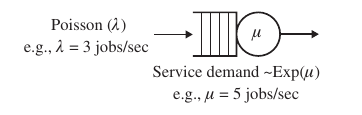
\includegraphics[scale=0.75]{images/queuing_02_01.png}
\end{figure}


In this case, the state of the CTMC is the number of jobs in the quene. We can draw an equivalent picture of the system as follows.


\begin{figure}[hbt!]
\centering
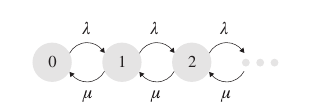
\includegraphics[scale=0.75]{images/queuing_02_02.png}
\end{figure}


We note the following

\begin{itemize}

\item The values $\lambda$ and $\mu$ are \emph{not} probabilities but rates.

\item Events like arrival of a new job, processing of a job change the state. When we are in a state $i \geq 1$, then the next event is an arrival or departure.

\item Let $X_A \sim \text{Exp}(\lambda)$ denote the time till the next arrival and $X_D \sim \text{Exp}(\mu)$ denote the time till next departure.

\item The state changes when the first event happens; i.e. with a time $X = min(X_A, X_D) \sim \text{Exp}(\lambda + \mu)$.

\item The probability when we leave state $i$ and arrive in state $i+1$ is $P(X_A < X_D) = \frac{\lambda}{\lambda + \mu}$.

\end{itemize}


What we are interested in are the limiting probabilties for being in state $i$,

\bee
\pi_i = \lim_{t \rightarrow \infty} P_{ij}(t)
\eee

The idea is to convert the DTMC from above into a DTMC and solve this for the limiting probabilities: The arrival and departures are independent and we model them by flipping two coins simultaneously every $\delta$-step (with $\delta \rightarrow 0$).

The first coin represents arrivals, is flipped every $\delta$-step, and returns "arrival" with probability $\lambda \delta$; with probability $(1-\lambda)\delta$ nothing happens.

In a similar spirit, the second coin represents departrues, is flipped every $\delta$-step, and returns "departure" with probability $\mu \delta$; with probability $(1-\mu)\delta$ nothing happens.

Now we can combine the outcome of the two (independent) coin flips

\begin{itemize}

\item With probability $\lambda \delta (1-\mu \delta)$, we get arrival and no departure.

\item With probability $(1 - \lambda \delta) \mu \delta$, we get no arrival and departure.

\item With probability $\lambda \delta \mu \delta$, we get arrival and departure.

\item With remaining probability $1 - \lambda \delta (1 - \mu \delta)-\mu\delta(1-\lambda \delta)$, we get no arrival and no departure.

\end{itemize}

The corresponding DTMC is shown below.

\begin{figure}[hbt!]
\centering
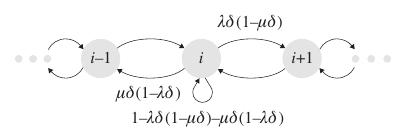
\includegraphics[scale=0.75]{images/queuing_02_03.png}
\end{figure}

We can solve this DTMC with observing $\delta^2 \rightarrow 0$ and arrive at the following set of equations

\begin{align*}
\pi_0 \lambda &= \pi_1 \mu \\
\pi_1(\lambda + \mu) &= \pi_0 \lambda + \pi_2 \mu \\
\pi_2(\lambda + \mu) &= \pi_1 \lambda + \pi_3 \mu
\end{align*}

Looking at the CTMC state diagram (replicated below), we can see that above equations are corresponding to it; however, $\mu$ and $\lambda$ are not probabilities.

The general approach to solving a CTMC is therefore to write the balance equations down and solving them.


\begin{figure}[hbt!]
\centering
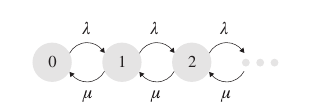
\includegraphics[scale=0.75]{images/queuing_02_02.png}
\end{figure}





%%% Local Variables:
%%% mode: latex
%%% TeX-master: "journal"
%%% End:
